\documentclass[a4paper, 12pt]{article}
\usepackage[english]{babel}
\usepackage[utf8]{inputenc}
\usepackage[T1]{fontenc}
\usepackage{lmodern}

\usepackage{url}
\usepackage{graphicx}

\usepackage{amsmath}
\usepackage{amsthm}
\usepackage{amsfonts}


\theoremstyle{definition}
\newtheorem{definicija}{Definicija}

\theoremstyle{plain}
\newtheorem{izrek}{Izrek}

% ne spreminjaj podatkov, ki vplivajo na obliko strani
\textwidth 15cm
\textheight 24cm
\oddsidemargin.5cm
\evensidemargin.5cm
\topmargin-5mm
\addtolength{\footskip}{10pt}
\pagestyle{plain}
\overfullrule=15pt % oznaci predlogo vrstico


% ukazi za matematicna okolja


% za stevilske mnozice uporabi naslednje simbole
\newcommand{\R}{\mathbb R}
\newcommand{\N}{\mathbb N}
\newcommand{\Z}{\mathbb Z}
\newcommand{\C}{\mathbb C}
\newcommand{\Q}{\mathbb Q}
\newcommand{\f}{\mathcal F}
\newcommand{\p}{\mathbb P}

% ukaz za slovarsko geslo
\newlength{\odstavek}
\setlength{\odstavek}{\parindent}


% naslednje ukaze ustrezno popravi
\newcommand{\program}{Finančna matematika} % ime studijskega programa: Matematika/Finan'cna matematika
\newcommand{\imeavtorja}{Tia Krofel, Brina Ribič, Matej Rojec} % ime avtorja
\newcommand{\imementorja}{dr. Aleš Ahčan} % akademski naziv in ime mentorja
\newcommand{\naslovdela}{VaR on option portfolio}
\newcommand{\letnica}{2022}


\begin{document}

% od tod do povzetka ne spreminjaj nicesar
\thispagestyle{empty}
\noindent{\large
UNIVERZA V LJUBLJANI\\[1mm]
FAKULTETA ZA MATEMATIKO IN FIZIKO\\[5mm]
\program\ -- 2.~stopnja}
\vfill

\begin{center}{\large
\imeavtorja\\[2mm]
{\bf \naslovdela}\\[10mm]
Seminarska naloga pri predmetu Upravljanje tveganj\\[1cm]
Mentor: \imementorja}
\end{center}
\vfill

\noindent{\large
Ljubljana, \letnica}
\pagebreak

\thispagestyle{empty}
\tableofcontents
\pagebreak

\section{Osnovno o opcijah}

Opcija je pogodba med nosilcem opcije (kupcem) in izdajateljem opcije
o nakupu oziroma prodaji osnovnega premoženja (temelja) po določeni ceni $K$ imenovani
izvršilna cena. Če opcija daje nosilcu pravico nakupa temelja, jo imenujemo nakupna opcija, če pa daje pravico prodaje,
jo imenujemo prodajna opcija. Glede na to, kdaj je možna izvršitev opcije, ločimo več vrst opcij.
Najbolj preprosta je evropska opcija, ki daje pravico izvršitve samo ob zapadlosti. Ameriška opcija
daje pravico izvršitve kadarkoli do vključno trenutka zapadlosti. Poznamo tudi druge vrste opcij, ki jih skupno imenujemo eksotične opcije.

Označimo s $t=0$ čas izadje opcije, s $t=T$ pa čas zapadlosti.
Naj bo $S_t$ cena osnovnega premoženja ob času $t\in [0,T]$.
Vrednost opcije za nosilca opcije je enaka razliki med ceno osnovnega premoženja v času
izvršitve in izvršilno ceno, če je zanj pozitivna. Sicer opcije ne izvrši in je njena
vrednost enaka $0$. Izplačilo evropske nakupne opcije ob času T je
\begin{equation}
    C_T = max\{S_T-K,0\},
\end{equation}
saj se mu v primeru, ko je $S_T<K$ ne splača izvršiti opcije, torej je njeno izplačilo $0$.
Izplačilo evropske prodajne opcije pa je enako 
\begin{equation}
    P_T = max\{0, K-S_T\}.
\end{equation}

Kupec opcije mora ob nakupu opcije plačati premijo. Kako visoka je ta premija, je precej komplicirano izračunati.
Premijo oziroma vrednost opcije bomo računali z Black-Scholesovim modelom. Cena evropske prodajne opcije ob času $t$ je 
\begin{equation}\label{prodajna}
    V_t = Ke^{-R(T-t)}\Phi(-d_2)-S_t\Phi(-d_1),
\end{equation}
kjer je
\begin{itemize}
    \item $K$ izvršilna cena opcije,
    \item $R$ netvegana obrestna mera,
    \item $S_0$ cena temelja ob času $0$.
\end{itemize}
Konstanti $d_1$ in $d_2$ izračunamo s formulama
\begin{equation}
    \begin{aligned}
        d_1 &= \frac{\ln(\frac{S_0}{K}e^{RT})+\frac{\sigma^2}{2}T}{\sigma\sqrt{T}},\\
    d_2 &= d_1-\sigma\sqrt{T}. 
    \end{aligned}
\end{equation}
Tu je $\sigma$ volatilnost donosov temelja. Podobno formulo dobimo za izračun premije evropske nakupne opcije
\begin{equation}\label{nakupna}
    V_t = S_t\Phi(d_1) - Ke^{-R(T-t)}\Phi(d_2).
\end{equation}

Glavna predpostavka v tem modelu je, da ima temelj zvezno neodvisno enako normalno porazdeljene donose.
Naš cilj bo oceniti tveganje opcij glede na temelj. To bomo naredili s t. i. grškimi parametri.

%While the type (put or call) and the underlying stock are self-evident and essentially standardized, the striking price and expiration date require more
%explanation. 

%Striking prices intervals are not hardcoded, they are detirmened on an exchange.
%They are generally spaced 5 points apart, but for expensive stock they and be 
%10 points or more apart andfFor cheaper stocks (i.e. less then \$35 per share)
%they can be 2.5 points apart. However these intervals can be altered, based on 
%market depth and liqudity.

% B-S model
% grki
% zaščitni portfelj

\section{Osnovno o VaR}

"Value at Risk" oziroma VaR je mera, ki je opredeljena kot največja potencialna sprememba v vrednosti portfelja pri določeni,
dovolj visoki stopnji zaupanja za vnaprej določeno časovno obdobje. Ponavadi je stopnja zaupanja $95\%$ ali $99\%$.
VaR nam pove, koliko lahko izgubim z $x\%$ verjetnostjo v nekem časovnem obdobju. Ponavadi se uporablja
krajše časovno obdobje, recimo dan, teden ali nekaj tednov.
To pomeni, če je VaR za neko sredstvo $100$ milijonov evrov v obdobju enega tedna s stopnjo zaupanja $95\%$,
potem je samo $5\%$ verjetnost, da bo vrednost sredstva padla za več kot $100$ milijonov evrov v katerem koli tednu.

Let us now give a formal definiton of value at risk. 
\begin{definicija}
Let $X$ be a random variable on a probability space $(\Omega, \f, \p)$ and $\alpha \in (0, 1)$.
VaR$_\alpha(X)$ is defined as the $(1-\alpha)$ quntile of -$X$. So:
$$
\textnormal{VaR}_\alpha(X) := - \inf \{ x \in \R \mid F_X(x) > \alpha \} = F^{-1}_{-X}(1-\alpha).
$$
\end{definicija}

Obstajajo trije osnovni pristopi, kako izračunati VaR. Lahko ga izračunamo analitično
s predpostavkami o porazdelitvah donosov za tržna tveganja, zraven pa moramo upoštevati variance
in kovariance med temi tveganji. VaR lahko ocenimo tudi s hipotetičnim portfeljem preko historičnih 
podatkov ali z Monte Carlo simulacijo. 

Nas bo zanimalo, kaj se zgodi, če imamo sredstvo, ki je izvedeni finančni instrument. V tem primeru moramo 
nekoliko modificirati VaR.
Recimo pri opcijah, moramo pri oceni tveganja upoštevati nelinarno gibanje cen (gamma učinek)
in posredna volatilnost (vega učinek). % implied volatilities
Za opcije bomo nelinearno gibanje cen ocenili analitično (delta-gamma) ali s simulacijo.


\subsection{Kako izračunamo VaR}

\subsubsection{Variančno-kovariančna metoda}

Variančno-kovariančna metoda je parametrična metoda, ki predpostavlja, da so donosi, 
kateri določajo vrednost portfelja,
porazdeljeni normalno. Slučajna spremenljivka je porazdeljena normalno s parametroma $\mu$ (povprečje)
in varianco $\sigma^2$ oziroma standardnim odklonom $\sigma$, če je gostota podana z 
\begin{equation}
    f(x) = \frac{1}{\sigma\sqrt{2\pi}}exp[-\frac{1}{2}(\frac{x-\mu}{\sigma})^2],
\end{equation}
kjer je $x\in \R$. Ta metoda je uporabna, ker je v celoti definirana samo z dvema parametroma. 
Hkrati nam zagotavlja direktne formule za izračun kumulativnih porazdelitvenih funkcij; velja namreč
\begin{equation}
    P(X<x) = \mu + \alpha_{cl}\sigma,
\end{equation}
kjer je $cl$ izbrana stopnja zaupanja (npr. $95\%$) in $\alpha_{cl}$ je standardna normalna spremenljivka pri izbrani stopnji zaupanja
(npr. $\alpha_{0.95}=1.645$). 

VaR za eno naložbo je potem enak
\begin{equation}
    VaR = MV\cdot \alpha_{cl} \cdot \sigma,
\end{equation}
kjer je $MV$ tržna vrednost temelja. Pri izračunu VaR za portfelj, ki je sestavljen iz več pozicij,
moramo upoštevati tudi diverzifikacije oziroma razpršitve naložb.
% dodaj še natančnejši opis
Pri opcijah se ta metoda izkaže za učinkovito, potrebno jo je le nekoliko modificirati. Ker je vrednost opcije odvisna od več dejavnikov 
ter imamo nelinearno povezavo med vrednostjo opcije in donosnostjo temelja, moramo izračunati še nekaj dodatnih parametrov, da bo rezultat korekten.

\subsubsection{Zgodovinska simulacija}
Zgodovinska simulacija omogoča zelo preprosto in intuitivno oceno VaR. Temelji na vrstnem redu opazovanih podatkov;
recimo, da imamo $100$ opažanj, potem je šesto po vrsti VaR pri stopnji zaupanja $95\%$. 
Zavedati pa se moramo, da lahko pride do večjih napak pri tem načinu izračuna VaR zaradi ekstremnih dogodkov, dolžine opazovanega obdobja, \dots
Prav tako ta metoda ni primerna za izračun nelinernega VaR oziroma 
za izračun VaR za opcije, saj je historične podatke za opcije težko dobiti in jih med seboj primerjati.

\subsubsection{Monte Carlo simulacija}
Monte Carlo simulacija je danes v praksi zelo uporabna saj je precej prilagodljiva za veliko različic VaR. 
Izkazalo se bo, da je uporabna tudi za izračun nelinearnega VaR.

\section{Nelinearen VaR}

Osnovna različica VaR predpostavlja linearno povezavo med donosi in spremembo vrednosti pozicije
oziroma da je relativna sprememba portfelja linearna funkcija donosa temelja (delnice, obveznice \dots)
Tu predpostavljamo, da imajo donosi vrednostnega papirja večrazsežno normalno porazdelitev.  

Vrednost pozicij pri izvedenih finančnih instrumentih je odvisna od vrednosti od nekega drugega vrednostnega papirja.
Pri opcijskih pozicijah je nelinearna povezava med spremembo vrednosti pozicije in donosom temelja. 
To lahko pojasnimo s preprosto opcijo na delnico. Cena opcije je $V(S_t,K,T,R,\sigma)$ v 
odvisnosti od cene delnice $S_t$ ob času $t$, izvršilne cene $K$, časa dospelosti $T$. 
Cena opcije je odvisna tudi od netvegane obrestne mere $R$ nekega vrednostnega papirja, ki ima enak
čas dospelosti kot opcija ter od standardnega odklona $\sigma$ cene temelja v časovnem obdobju opcije. 
Zato moramo uporabiti drugačen pristop za računanje VaR za portfelj iz opcij. 

\begin{figure}\label{payoff}
    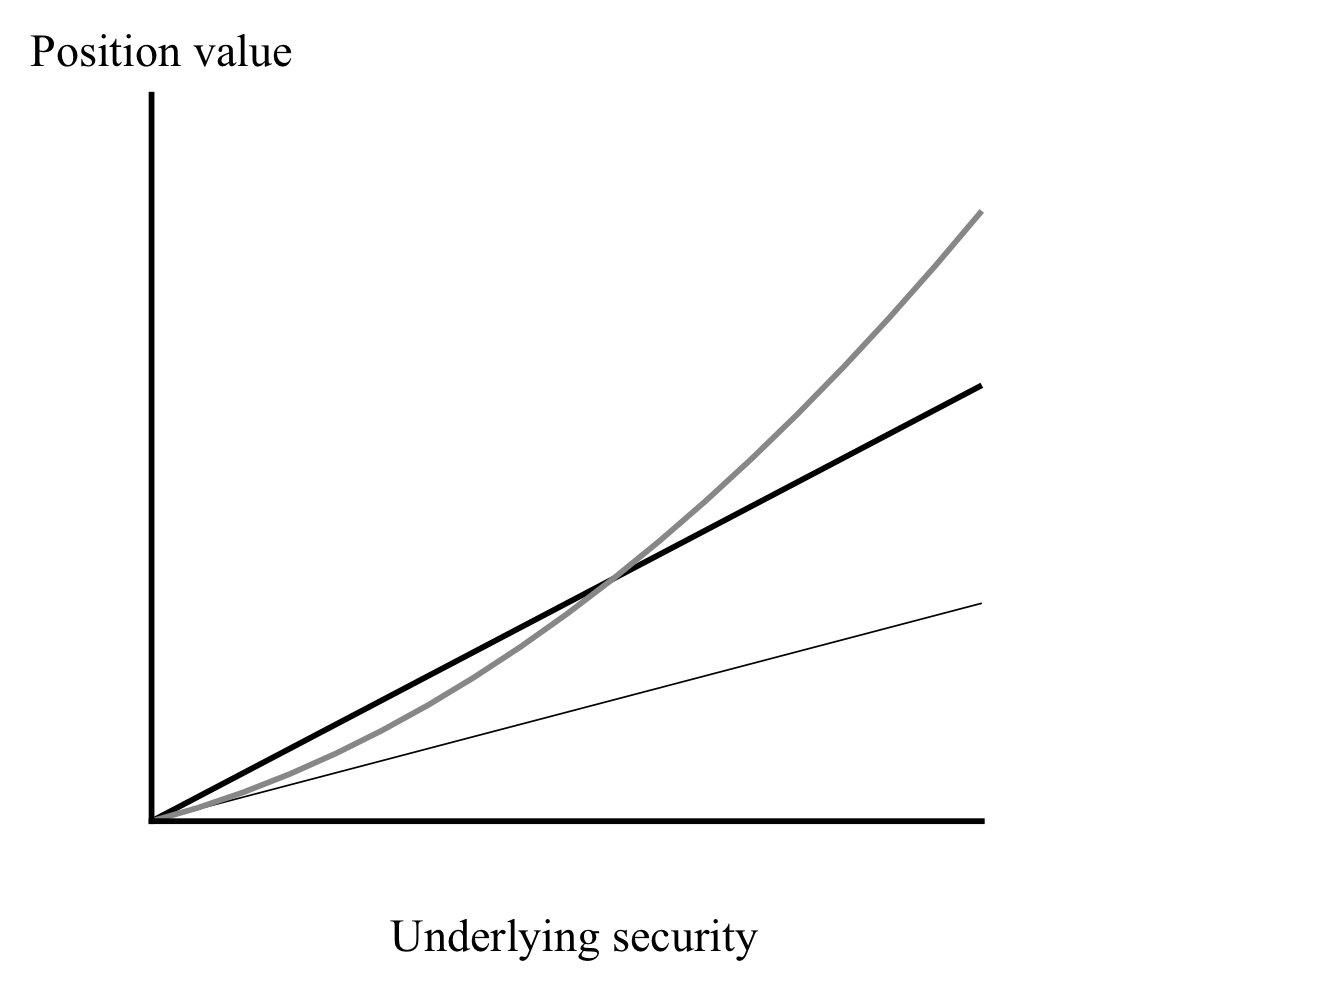
\includegraphics[width=0.7\textwidth]{payoff.jpg}
    \caption{Linearna in nelinearna funkcija izplačila.}
\end{figure}

Na sliki \ref{payoff} je prikazana vrednost pozicije glede na temelj. 
Ravni črti predstavljata linearno zvezo med vrednostjo pozicije in vrednostjo temelja. 
Vrednost evropske opcije (nakupne ali prodaje) bomo izrazili z "delta". To pomeni, da zveza
med vrednostjo pozicije in vrednostjo temelja ne bo več linearna ampak nelinearna. Na grafu to 
predstavlja siv graf funkcije. Opazimo, da ni več linearna funkcija.
V primeru, ko je zveza linearna, je "delta" $-1$ ali $1$. Če pa je "delta" katero koli drugo število
med $-1$ in $1$, govorimo o nelinearni povezavi med vrednostjo pozicije in vrednostjo temelja.
Dodatno potrebujemo parameter "gamma", s katerim bomo definirali konveksnost funkcije. Pri linearnih zvezah
je "gamma" vedno enak $0$ in imajo konstanten naklon. Pri nelinearnih zvezah, recimo pri opcijah, pa je 
"gamma" vedno neničelno nenegativno število. Od tod izhajajo različni pristopi za računanje nelinearnega VaR.


Pri vseh različicah še vedno predpostavljamo, da so donosi vrednostnih papirjev porazdeljeni normalno. 
Dodatno dopuščamo nelinearno zvezo med vrednostjo pozicije in donosi temelja. Natančneje, dovoljujemo gama učinek,
torej da relativna sprememba portfelja iz derivativov (v našem primeru opcij) ni več normalno porazdelja. 
Zaradi tega ne moremo več VaR definirati kot 1.65 krat standardni odklon portfelja. Namesto tega VaR 
izračunamo v dveh glavnih korakih. Najprej izračunamo prve štiri momente porazdelitve donosa portfelja, tj.,
povprečje, standardni odklon, \textbf{skewness}, \textbf{kurtosis}. Potem poiščemo 
porazdelitev, ki ima enake prve štiri momente kot porazdelitev donosa portfelja in izračunamo peti 
percentil (ali prvi, odvidno od problema). Od tod dobimo VaR.
\newpage

\section{The Greeks}


As we want to calculate the theoretical value of an 
option and understand its changes in response to 
various factors, we now take a closer look at some of the 
"Greeks". \\

In the context of options trading, they present a 
set of sensitivity measures, usually computed 
using the Black-Scholes formula. 

And while they are relevant to hedging strategies 
(which is especially true for delta and gamma),
these derivatives are typically calculated because 
they can give us an idea about how rapidly 
the value of our portfolio is effected when there is a 
change in one of the parameters underlying the 
Black-Scholes model.



\subsection{The Delta}

The delta of an option ($\Delta$) 
is a theoretical estimate 
of how much an option price would change 
relative to a change in the price of the underlying asset.
It expresses the amount by which an option changes for a 1-point 
move in the underlying security.

Using symbols as defined in sections 1 and 3, 
we can present this first-order sensitivity of an option
with respect to the underlying price 
as 
$$
\Delta = \frac{\partial V}{\partial S},
$$ 
where $\Delta\in [0,1]$ for calls and $\Delta\in [-1,0]$ for puts.
Stated in another way, it is the percentage of any
stock price change that will be reflected in the change of the 
price of the option. 

Let's look at an example. We will assume that a Stock A January 50 call has a delta of 0.25 
with Stock A at a current price of 49. This means that the call will move 
25\% as fast as the stock will move. So, if Stock A
jumps to 51, a gain of 2 points, then the January 50 call can be expected to increase
in price by 0,5 point (25\% of the stock increase).

There is one other interpretation of the delta that is perhaps of less practical
use, but is still worth mentioning.
If we ignore the sign of the delta (positive for
calls, negative for puts),
the delta is often also thought of as the probability of the
option being in-the-money at expiration. 
That is, if Stock A price is 50 and the January 55 call has
a delta of 0.40, then there is a 40\% probability that Stock A will be over 55 at January
expiration. 
Of course, this is only an approximation of the probability because
interest rates and dividends may distort this interpretation.

If an option's 
delta is equal to zero, the 
option price barely moves when the price of the 
underlying asset changes. 
If an option's delta is positive, then 
that option's price will increase 
when the underlying asset's price 
increases, while negative delta indicates a decrease
in the option price as the underlying 
asset's price increases. 

Put deltas are expressed as negative numbers to indicate that put prices move
in the opposite direction from the underlying security. 
Deltas of out-of-the-money options are smaller 
compared to in-the-money options, going toward 0 as the option becomes
very far out-of-the-money. 

This means that short calls and long puts have 
a delta with values between -1 and 0, while 
long calls and short puts have a delta
with values ranging between 0 and 1.
If an option's delta is very close to -1 or 1 
then it is deeply in-the-money
(depending on whether it is put or call).
% Also means it's deep in the money 
In case of a european call option, 
using the above formula would give us 
its delta equal to $\Phi(d_1)$. 

However, while small changes in the underlying asset's
price do change the option price by approximately delta,
such approximations get less and less reliable as 
the asset's price change gets greater.

The volatility of the underlying stock has an effect on delta also. If the stock is not
volatile, then in-the-money options have a higher delta, and out-of-the-money
options have a lower delta.


\subsection{The Gamma}

Gamma, or second-order sensitivity of an option 
with respect to the underlying asset's price, 
measures the change in an option's delta relative to changes 
in the underlying asset price. 
Simply stated, the gamma is how fast the delta changes with respect to changes in the
underlying stock price.

We can calculate it as follows:
$$
\Gamma = \frac{\partial^2 V}{\partial S^2}.
$$

We have already stated before that the delta of a call option 
increases as the call moves more from out-of-the-money to in-the-money.
The gamma is in fact only a precise measurment of how fast the delta is 
increasing.

Let's look at an example. We will assume that a Stock B January 50 call has a delta of 0.25
and a gamma of 0.05, with Stock B at a current price of 49. 
This means that if the call will move one point up to 50
then the delta will change (increase) from 0.25 to 0.30.

Let's look at one more example. We will assume that a Stock B January 50 call has a 
delta of 0.25 and a gamma of 0.05, with Stock B at a current price of 49. 
This means that if the call will move two point up to 51
then the delta will change (increase) from 0.25 to 0.35.,
because of the gamma.
In this case the delta increased by 0.10.

Obviously, the above example is flawed, as the
delta cannot keep increasing by 0.05 each time 
Stock B gains another point in price, for it will eventually exceed 1.00,
and we know that for call options the Delta has an upper bound of 1.
Therfore it is obvious that the gamma has to change.
In general, the gamma is at its maximum point when the stock is near the strike of the
option.
As the stock moves away from the strike in either direction, the gamma
decreases, approaching its minimum value of zero. 

Let's look at an example of the stated above. 
We will assume that a Stock B January 50 call has a 
delta of almost 0 at a current price of 25  Stock B per share.
If the price of Stock B moves up one point to 26, 
the call is still so far out-of-the-money that the delta
will still be zero.  Thus, the gamma of this call is zero, 
since the delta does not change when the stock increases in price by a point.

Higher values of an option's gamma indicate that very small 
price change of the underlying asset could lead to 
big changes in the option's delta value.

Options that are at-the-money (when their strike prices 
are equal to the price of underlying asset) have the 
highest gamma values as the delta of such an option is 
very sensitive to price change of the underlying asset. 
As this underlying asset's price moves further away 
from the option's strike price in either direction, 
gamma values decrease. 
Long options, whether puts or calls, have positive gamma, while short options
have negative gamma. Thus, a strategist with a position that has positive gamma has
a net long option position and is generally hoping for large market movements.
Conversely, if one has a position with negative gamma, it means he has shorted
options and wants the market to remain fairly stable. 
 
Another property of gamma is useful to know as well. 
As expiration nears, the gamma of at-the-money options increases dramatically.  
Consider an option with a day
or two of life remaining. If it is at-the-money, the delta is approximately 0.50.
However, if the stock were to move 2 points higher, the delta of the option would jump 
to nearly 1.00 because of the short time remaining until expiration. Thus, the gamma
would be roughly 0.25. as compared to much smaller values of gamma for at-the-money options with several
weeks or months of life remaining.
Contrary out-of-the-money options display a different relationship between gamma and
time to expirery. An out-of-the-money option that is about to expire has a very small
delta, and hence a very small gamma.

The volatility of the underlying security also plays a part in gamma. 
At-themoney options on less volatile securities will have higher gammas than similar options
on more volatile securities. 

\subsection{The Theta}

Measuring an options's sensitivity to time, 
theta tell us how susceptible is an option's value 
to the passage of time. 

Earlier in this section, we have seen how delta and gamma
values of an option are effected by the price movement 
of the underlying asset in comparison to the option price.

In case of theta, we look at the effect of time decay 
on an option. All other factors being equal, the theta of 
an option represents the amount by which the option's value 
will decrease each day. It is calculated as the following 
derivative:
$$
\Theta = \frac{\partial V}{\partial t}.
$$

Its value is usually negative - with each passing day, 
an option's potential for profitability drops.
As an option gets closer to its expiration date, 
the rate of time decay gets faster.

We understand an option's intrinsic value as a measure 
of the actual value of the strike price compared to the 
current market price and its extrinsic value as a measure 
of the part of the premium that is not defined by 
the intrinsic value, namely the value of being able to 
hold the option and the opportunity for the option to gain 
value as the underlying asset moves in price. Consequentially,
the closer that an option is to expiration, the smaller 
its extrinsic value becomes - at the expiration date, 
an option's extrinsic value is zero.

Theta is then the measure that determines the decline in 
an option's extrinsic value over time.

Long positions generally have a negative theta while 
short positions have a positive one. 


\subsection{The Vega}

There is no letter in the Greek alphabet called ``vega''.
Thus, some strategists, prefer to use a real Greek letter, 
``tau'', to refer to this risk measure, however 
we will use ``vega''.
Just as option values are sensitive to changes in the underlying price (delta) and
to the passage of time (theta), they are also sensitive to changes in volatility. 
Vega measures sensitivity to volatility. 
Vega is the derivative of the option value with respect to the volatility of the underlying asset.
Volatility in this sense is a measure of how quickly the underlying security moves around. 
We usually calculate it as the standard deviation of stock prices over some
period of time, generally annualized.
A stock with higher volatility is therfore more volatile.
It is calculated as the following derivative:
$$ 
\mathcal{V}  = \frac{\partial V}{\partial \sigma}
$$


Vega is the amount by which the option price changes when the
volatility changes. Vega is therfore always a positive number, whether it refers to
a put or a call. 

It is logical that more volatile stocks have more expensive options. 
Increasing volatility, means that the price of an option will rise. 
Falling volatility, means that the price of an option will fall. 
The vega is merely an attempt to quantify how much the
option price will increase or decrease as the volatility moves, 
all other factors being equal. 

Let's look at company D is at 49, and the January 50 call is selling for 3.50. The
vega of the option is 0.10, and the current volatility of company D is 30\%.
If the volatility had instead decreased by 1 percent to 29\%, then the January 50
call would have decreased to 3.40 (a loss of 0.10, the amount of the vega).
If the volatility increases by one percentage point or 1 \% to 31 \%, then the vega
indicates that the option will increase in value by 0.10, to 3.60. 

Vega is greatest for at-the-money options and approaches zero as the option is
deeply in- or out-of-the-money. Again, this is common sense, since a deep in- or out
of-the-money option will not be affected much by a change in volatility. In addition,
for at-the-money options, longer-term options have a higher vega than short-term
options. An at-the-money option with on
day to expiration will not be overly affected by any change in volatility, due to its
pending expiration. However, a three-month at-the-money option will certainly be
sensitive to changes in volatility.

Vega does not directly correlate with either delta or gamma. One could have a
position with no delta and no gamma (delta neutral and gamma neutral) and still have
exposure to volatility. This does not mean that such a position would be undesirable;
it merely means that if one had such a position, they would have removed most of the
market risk from his position and would be concerned only with volatility risk. 

\section{Delta-Gamma-Theta Approach}

Let us now take a closer look 
at the methodology for using  
the delta, gamma and theta of 
options in the VaR calculation. 


Overall, incorporating these greeks into the VaR calculation 
can provide a more accurate estimate of the risk of 
loss on a portfolio of options.

By taking into account the price sensitivity and time 
decay of each option, this analytical approach can better 
reflect the potential impact of market movements on 
the portfolio's value. Based on the theoretical 
background covered in section 4, the importance of 
each of the three greeks used for this VaR calculation is as follows:

\begin{itemize}
    \item Delta is important for VaR analysis 
    because it estimates the potential change 
    in the option's value associated with a 
    unit shift in the underlying asset's price;
    \item Gamma plays an increasingly important role in 
    VaR calculations as the underlying asset price 
    fluctuates more significantly;
    \item Theta is an important consideration for VaR 
    analysis, because time decay is a major factor
    in the approximation of the overall risk of the portfolio.
\end{itemize}

For example, 
a portfolio with a high gamma may be 
more sensitive to changes in the 
underlying asset's price, 
while a portfolio with a high theta 
may be more sensitive to the passage 
of time.\\


The simplest approximation using greeks would estimate changes 
in the option value with a linear model - in this case, we would 
only use delta-approximation. This would be a relatively accurate 
model only when the price of the underlying asset would not undergo any 
significant changes. The reason for this is in delta being a linear 
approximation of a non-linear relationship between option value and underlying 
asset's price. 

This may be improved with inclusion of gamma, which also accounts for 
non-linear effects of change as it introduces skewness into the price distribution.


Finally, we add theta into the equation to improve the accuracy of the calculation 
with inclusion of the time decay.\\

And while this approach does not necessitate any simulations,
we do need (besides the delta, gamma and theta 
parameters) a covariance matrix and position values. 





\subsection{Limitations}

There are, however, some limitations to the usage of such an approach
when calculating VaR. 

Namely, it may not be suitable for options portfolios with more complex 
risk profiles, such as those with illiquid assets. 
It is also subject to model risk (like any statistical model),
so it may produce inaccurate results due to errors in the 
assumptions or parameters used in the model.

And even as it does provide, as stated above, 
a more comprehensive and accurate assessment of the risk 
of loss on a portfolio of options, it may still not be 
sufficient to capture the full range of risks faced by 
an options portfolio.


\end{document}